
%(BEGIN_QUESTION)
% Copyright 2012, Tony R. Kuphaldt, released under the Creative Commons Attribution License (v 1.0)
% This means you may do almost anything with this work of mine, so long as you give me proper credit

Write the equation describing the behavior of this pneumatic controller, assuming identical bellows all around:

$$\includegraphics[width=15.5cm]{i01666x01.eps}$$

Next, identify at least two different ways to {\it adjust the bias} of this proportional-only pneumatic controller, if you could change any aspect of its construction:

\vskip 20pt \vbox{\hrule \hbox{\strut \vrule{} {\bf Suggestions for Socratic discussion} \vrule} \hrule}

\begin{itemize}
\item{} Explain why it is important to determine whether the mechanism is {\it force-balance} or {\it motion-balance} in your analysis.
\item{} A common mistake students make when sketching a pneumatic mechanism is to place the orifice (restrictor) between the output tube and the nozzle.  Explain why this is wrong.
\end{itemize}

\underbar{file i01666}
%(END_QUESTION)





%(BEGIN_ANSWER)

Based strictly off the dimensions shown in the diagram, it would first appear that the controller's gain should be 0.6875 (equal to $2.4 \over 3.5$) and that therefore the controller equation should be:

$$m = 0.6857 (\hbox{PV} - \hbox{SP}) + b$$

However, on closer analysis and inspection of the shorter lever coupling the PV and SP bellows together, it is possible to see that the gain is only {\it half} this amount:

$$m = 0.3429 (\hbox{PV} - \hbox{SP}) + b$$

Explain why this is!

%(END_ANSWER)





%(BEGIN_NOTES)

Ways to adjust the bias:

\begin{itemize}
\item{} Move position of nozzle (vertically) closer to or farther away from lever
\item{} Change link length between bellows and lever
\end{itemize}






\vfil \eject

\noindent
{\bf Summary Quiz:}

Suppose the nozzle were shifted to the left along the lever (further away from the output bellows).  What effect would this have on the controller's behavior?

$$\includegraphics[width=15.5cm]{i01666x02.eps}$$

\begin{itemize}
\item{} The bias would increase
\vskip 5pt 
\item{} The gain would increase
\vskip 5pt 
\item{} The action would switch to become direct-acting
\vskip 5pt 
\item{} The action would switch to become reverse-acting
\vskip 5pt 
\item{} The gain would decrease
\vskip 5pt 
\item{} The bias would decrease
\end{itemize}

%INDEX% Control, proportional: pneumatic motion-balance controller

%(END_NOTES)


